
\documentclass[12pt]{amsart}
%\usepackage{geometry} % see geometry.pdf on how to lay out the page. There's lots.
\usepackage{graphics}
\usepackage{graphicx}
\usepackage{fullpage}
%\geometry{a4paper} % or letter or a5paper or ... etc
% \geometry{landscape} % rotated page geometry
\usepackage{tikz}
\usetikzlibrary{arrows}
\usetikzlibrary{positioning}


\begin{document}

\begin{center}
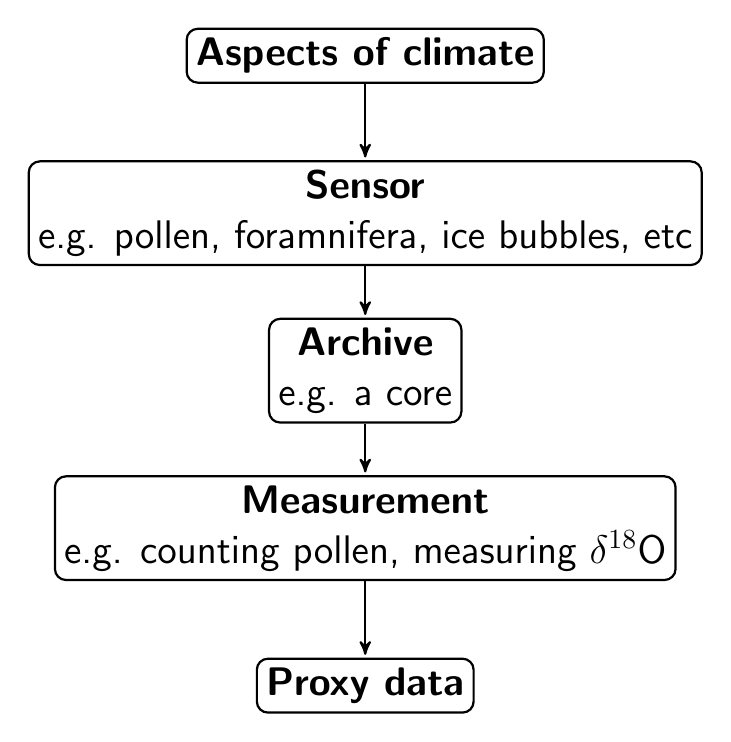
\begin{tikzpicture}[->,>=stealth',shorten >=1pt,auto,node distance=2cm,
                    thick,main node/.style={rectangle,rounded corners,draw,font=\sffamily\Large}]

  \node[main node](1) {\textbf{Aspects of climate}};
  \node[main node](2) [below of=1,align=center] {\textbf{Sensor}\\e.g. pollen, foramnifera, ice bubbles, etc};
  \node[main node](3) [below of=2,align=center] {\textbf{Archive}\\e.g. a core};
  \node[main node](4) [below of=3,align=center] {\textbf{Measurement}\\e.g. counting pollen, measuring $\delta^{18}$O};
  \node[main node](5) [below of=4] {\textbf{Proxy data}};
  
  \path[every node/.style={font=\sffamily\small}]
    (1) edge node [right] {} (2)
	(2) edge node [right] {} (3)
	(3) edge node [right] {} (4)
	(4) edge node [right] {} (5);
\end{tikzpicture}
 
\end{center}
	


\end{document}
